\documentclass[t,xcolor={svgnames}]{beamer}

\mode<presentation>
\usetheme{Warsaw}
\useoutertheme{infolines} 

\usepackage{fontspec}
\usepackage{lmodern}
\usepackage{amsmath}
\usepackage{amsfonts}
\usepackage{bbm}
\usepackage{bm}
\usepackage[font=small,labelfont=bf]{caption} % Required for specifying captions to tables and figures
\usepackage{nicefrac}
\usepackage{color}
\usepackage{perpage}
\usepackage{multirow}
\usepackage{multicol}
\usepackage{adjustbox}
\usepackage{tikz}
\usepackage{tikz-dependency}
\usepackage{tikz-qtree}
\usepackage{tikz,pgfplots,pgfplotstable}
\usetikzlibrary{arrows.meta,graphs,graphs.standard,graphdrawing,quotes,shapes}
\usegdlibrary{layered,trees}

\tikzset{
  invisible/.style={opacity=0},
  visible on/.style={alt={#1{}{invisible}}},
  alt/.code args={<#1>#2#3}{%
    \alt<#1>{\pgfkeysalso{#2}}{\pgfkeysalso{#3}} % \pgfkeysalso doesn't change the path
  },
}

\captionsetup{labelformat=empty}
\newcommand{\parser}[1]{TUPA\textsubscript{#1}}

\newfontfamily\hebfont[Script=Hebrew, Scale=MatchUppercase]{FreeSans}
\newcommand{\heb}[1]{\bgroup\textdir TRT\hebfont #1\egroup}

\makeatletter
\pgfdeclareshape{vector}{
      \inheritsavedanchors[from={rectangle}]
      \inheritbackgroundpath[from={rectangle}]
      \inheritanchorborder[from={rectangle}]
      \foreach \x in {center,north east,north west,north,south,south east,south west,east,west}{
        \inheritanchor[from={rectangle}]{\x}
      }

    \backgroundpath{
      \pgftransformshift{\pgfpoint{-16pt}{-4pt}}
          \draw[rounded corners=2pt] (0,0) rectangle (32pt,8pt);
    }

    \beforebackgroundpath{
      \draw[step=8pt,help lines,-] (8pt,.1pt) grid (24pt,7.9pt);
    }
}
\pgfdeclareshape{vector}{
      \inheritsavedanchors[from={rectangle}]
      \inheritbackgroundpath[from={rectangle}]
      \inheritanchorborder[from={rectangle}]
      \foreach \x in {center,north east,north west,north,south,south east,south west,east,west}{
        \inheritanchor[from={rectangle}]{\x}
      }

    \backgroundpath{
      \pgftransformshift{\pgfpoint{-16pt}{-4pt}}
          \draw[rounded corners=2pt] (0,0) rectangle (32pt,8pt);
    }

    \beforebackgroundpath{
      \draw[step=8pt,help lines,-] (8pt,.1pt) grid (24pt,7.9pt);
    }
}
\makeatother

\MakePerPage{footnote}

% Outline slides
\AtBeginSection
{\begin{frame} \frametitle{Outline} \tableofcontents[currentsection,currentsubsection] \end{frame}}
\AtBeginSubsection
{\begin{frame} \frametitle{Outline} \tableofcontents[currentsection,currentsubsection] \end{frame}}


\begin{document}


\title[]{Universal Semantic Parsing with Neural Networks}
\author{Daniel Hershcovich}
\institute[]{PhD Lecture}
\date{February 5, 2019}

\begin{frame}
\titlepage
\end{frame}

\begin{frame}
\frametitle{Natural Language Processing: What's It Good For?}
\onslide<2>{Machine translation:}
\begin{center}
\onslide<2,5>{
  \fbox{After graduation, John moved to Copenhagen}

  $\downarrow$
}

\only<2,4>{
  \fbox{\heb{ג'ון עבר לקופנהגן אחרי שסיים את הלימודים}}
}
\only<3,5->{
  \fbox{\heb{\underline{\heb{ג'ון}} עבר ל\underline{\heb{קופנהגן}} אחרי שסיים את הלימודים}}
}
\end{center}

\vspace{-7mm}
  
\only<3>{
  \vspace{-5mm}

  Named entity \\
  recognition:

  \hspace{71mm} $\downarrow$ \hspace{12mm} $\downarrow$

  \hspace{65mm} Location \hspace{2mm} Person
}

\only<4>{
  Text \\
  simplification:
  
  \vspace{-1cm}
}
  
\only<4->{  
  \begin{center}
  $\downarrow$
  
  \fbox{\heb{ג'ון סיים את הלימודים. ג'ון עבר לקופנהגן.}}
  \end{center}
}

\only<5->{
  Sequence-to-sequence sometimes works, but lacks inductive bias.

  \begin{center}
    \begin{tikzpicture}[->]
    \tikzstyle{main}=[circle, minimum size=7mm, draw=black!80, node distance=12mm]
    \foreach \i in {1,3,7,9} {
        \node[main, fill=white!100] (h\i) at (\i,0) {};
        \node[main, fill=white!100] (o\i) at (\i.5,2) {};
    }
    \node (h5) at (5.5,0) {$\ldots$};
    \node (o5) at (5.5,2) {$\ldots$};
    \foreach \current/\next in {1/3,3/5,5/7,7/9} {
        \path (h\current) edge (h\next);
        \path (o\current) edge (o\next);
    }
    \foreach \i in {1,3,7,9} {
      \foreach \j in {1,3,7,9} {
        \path[gray!50] (h\i) edge (o\j);
      }
    }
    \end{tikzpicture}
  \end{center}
}

\end{frame}

\begin{frame}
\frametitle{Linguistic Structured Representations}
Model explicit relations between words or concepts.

\vfill

Example: {\color{DarkBlue}syntactic}/{\color{DarkRed}semantic} bi-lexical dependencies.

\vfill

    \begin{adjustbox}{center}
    \begin{dependency}[line width=1.5pt]
        \begin{deptext}[column sep=1.5em,ampersand replacement=\^,font=\rmfamily]
          After \^ graduation \^ , \^ John \^ moved \^ to \^ Copenhagen \\
        \end{deptext}
        \depedge[edge below,draw=DarkRed,edge unit distance=3ex]{1}{2}{ARG2}
        \depedge[edge below,draw=DarkRed,edge unit distance=3ex]{5}{4}{ARG1}
        \depedge[edge below,draw=DarkRed,edge unit distance=2ex, edge end x offset=-2pt]{1}{5}{ARG1}
        \deproot[edge below,draw=DarkRed,edge unit distance=3ex]{5}{top}
        \depedge[edge below,draw=DarkRed,edge unit distance=4ex, edge start x offset=-1pt, edge end x offset=3pt]{5}{7}{ARG2}
        \depedge[edge below,draw=DarkRed,edge unit distance=3ex, edge end x offset=5pt]{6}{5}{ARG1}
        \depedge[edge below,draw=DarkRed,edge unit distance=3ex]{6}{7}{ARG2}
        \depedge[draw=DarkBlue,edge unit distance=3ex]{2}{1}{case}
        \depedge[draw=DarkBlue,edge unit distance=3ex]{2}{3}{punct}
        \depedge[draw=DarkBlue,edge unit distance=3ex]{5}{4}{nsubj}
        \depedge[draw=DarkBlue,edge unit distance=3ex, edge end x offset=-2pt]{5}{2}{obl}
        \depedge[draw=DarkBlue,edge unit distance=3ex]{7}{6}{case}
        \deproot[draw=DarkBlue,edge unit distance=4ex]{5}{root}
        \depedge[draw=DarkBlue,edge unit distance=4ex]{5}{7}{obl}
    \end{dependency}    
    
    \end{adjustbox}
\end{frame}

\begin{frame}
    \frametitle{Semantic Representations}
Abstract away from detail that does not affect meaning:
\begin{center}
    \fbox{\textrm{rest}} $\approx$ \fbox{\textrm{take a break}}
    
    \vspace{1cm}
    
    \fbox{\textrm{graduation}} $\approx$ \fbox{\heb{סיים את הלימודים}}
\end{center}
\end{frame}

\begin{frame}
    \frametitle{Semantic Representations}

      \begin{flushright}
        \scalebox{.6}{
\begin{tikzpicture}[level distance=2cm, sibling distance=25mm, ->, draw=Indigo]
    \node[font=\bf\sffamily\Huge,Indigo] at (-3,0) {UCCA};
    \node (ROOT) [fill=Indigo, circle] {}
      child {node (After) {After} edge from parent node[left] {L\;}}
      child {node (graduation) [fill=Indigo, circle] {}
      {
        child {node {graduation} edge from parent node[left] {P}}
      } edge from parent node[left] {H} }
      child {node {,} edge from parent node[right] {U}}
      child {node (moved) [fill=Indigo, circle] {}
      {
        child {node (John) {John} edge from parent node[left] {A}}
        child {node {moved} edge from parent node[left] {P}}
        child {node [fill=Indigo, circle] {}
        {
          child {node {to} edge from parent node[left] {R}}
          child {node {Copenhagen} edge from parent node[left] {C}}
        } edge from parent node[left] {A} }
      } edge from parent node[right] {H} }
      ;
    \draw[dashed,->] (graduation) to node [auto] {\scriptsize A} (John);
\end{tikzpicture}
        }
      \end{flushright}
    
    \vspace{-23mm}
    
    \scalebox{.6}{
\begin{tikzpicture}
\node[font=\bf\sffamily\Huge,DarkGreen] at (0,6) {AMR};
\graph[layered layout, sibling distance=4cm, layer distance=2cm, nodes={ellipse,draw=DarkGreen}, edges={nodes={sloped}, DarkGreen}]{
a4 Copenhagen[as={Copenhagen}];
a2 John[as={John}];
a1[as={person}];
a0[as={move-01}];
a3[as={city}];
a2[as={name}];
a5[as={after}];
a4[as={name}];
a6[as={graduate-01}];

a1 ->  ["name"' above] a2;
a0 ->  ["ARG0"' above] a1;
a0 ->  ["ARG2"' above] a3;
a0 ->  ["time"' above] a5;
a3 ->  ["name"' above] a4;
a2 ->  ["op1"' above] a2 John;
a5 ->  ["op1"' above] a6;
a4 ->  ["op1"' above] a4 Copenhagen;
};
\draw[->, above, DarkGreen] (a6) to node[sloped] {ARG0} (a1);
\end{tikzpicture}
      }
    \vspace{-15mm}
    
    \begin{flushright}
    \begin{minipage}{.01\textwidth}
    {\color{DarkRed}\bf\sffamily\Large DM}
    \end{minipage}
    \begin{minipage}{.6\textwidth}
        \rmfamily
        \scalebox{.7}{
\begin{dependency}[theme=simple,edge style={-{Latex[length=2mm]}, color=DarkRed},
            text only label, label style={above, color=DarkRed, font=\bf\ttfamily}, font=\small]
    \begin{deptext}[column sep=1em,ampersand replacement=\^]
	After \^ graduation \^ , \^ John \^ moved \^ to \^ Copenhagen \\
    \end{deptext}
    \deproot{5}{top}
    \depedge{1}{2}{ARG2}
    \depedge{1}{5}{ARG1}
    \depedge{5}{4}{ARG1}
    \depedge{6}{5}{ARG1}
    \depedge{6}{7}{ARG2}
\end{dependency}
    }
    \end{minipage}
    \end{flushright}
\end{frame}


\section{Background: The UCCA Semantic Representation Scheme}

\begin{frame}
\frametitle{Universal Conceptual Cognitive Annotation (UCCA)}
Supports rapid and intuitive annotation of linguistic semantic phenomena. \\
\onslide<2->{
  Cross-linguistically applicable and stable \cite{sulem2015conceptual}.
}

\vfill

\begin{adjustbox}{center}
            \begin{tikzpicture}[level distance=7mm, sibling distance=6mm,
                every node/.append style={font=\rmfamily},
            	every circle node/.append style={fill=Indigo}]
                \begin{scope}[frontier/.style={distance from root=23mm},
                    edge from parent path={(\tikzparentnode.center)
                	.. controls +(0,-.25) and +(0,.25) .. (\tikzchildnode.north)},
                    edge from parent/.append style={nodes={font=\scriptsize}}]
                \Tree [.\node [circle] (root u) {};
                  \edge node [auto=right]{L}; \node (After u) {After};
                  \edge node[auto=left]{H};
                  [.\node [circle,xshift=8mm](graduation John u) {};
                    \edge node[auto=right]{P}; \node (graduation u) {graduation};
                  ]
                  \edge node[auto=left]{H};
                  [.\node [circle](John moved to Copenhagen u) {};
                    \edge node[auto=right]{A}; \node (John u) {John};
                    \edge node[auto=left]{P}; \node (moved u) {moved};
                    \edge node[auto=left]{A};
                    [.\node [circle](to Copenhagen u) {};
                      \edge node[auto=right]{R}; \node (to u) {to};
                      \edge node[auto=left]{C}; \node (Copenhagen u) {Copenhagen};
                    ]
                  ]
                ]
                \draw[dashed] (graduation John u) to node[auto] {\scriptsize A} (John u);
                \end{scope}
                \onslide<2->{
                  \begin{scope}[xshift=2cm,yshift=-58mm,grow'=up,level distance=9mm,
                      sibling distance=4mm, frontier/.style={distance from root=19mm},
                      edge from parent path={(\tikzparentnode.center) ..
                      controls +(0,.25) and +(0,-.25) .. (\tikzchildnode.south)},
                      edge from parent/.append style={nodes={font=\scriptsize}}]
                  \Tree [.\node [circle] (rootd) {};
                    \edge node[auto=left]{H};
                    [.\node [circle,xshift=-5mm] (John siyem et halimudim d) {};
                      \edge node[auto=left]{P}; \node (halimudim d) {\heb{הלימודים}};
                      \edge node[auto=left]{F}; \node (et d) {\heb{את}};
                      \edge node[auto=right]{D}; \node (siyem d) {\heb{שסיים}};
                    ]
                    \edge node [auto=left,anchor=south east]{L}; \node (ahrei d) {\heb{אחרי}};
                    \edge node[auto=right]{H};
                    [.\node [circle] (hu avar lecopenhagen d) {};
                      \edge node[auto=left,anchor=south east]{A}; \node (lecopenhagen d) {\heb{לקופנהגן}};
                      \edge node[auto=left]{P}; \node (avar d) {\heb{עבר}};
                      \edge node[auto=right]{A}; \node (John d) {\heb{ג'ון}};
                    ]
                  ]
                  \draw[dashed] (John siyem et halimudim d) to[out=-15,in=-150] node[above] {\scriptsize A} (John d);
                  \end{scope}
                }\onslide<3>{
                  \begin{scope}[dashed,thick]
                    \draw[DarkRed] (After u) to[out=-45,in=135] (ahrei d);
                    \draw[DarkGreen] (graduation u) to[out=-90,in=100] (John siyem et halimudim d);
                    \draw[DarkBlue] (John u) -- (John d);
                    \draw[orange] (moved u) to[out=-30,in=90] (avar d);
                    \draw[magenta] (to Copenhagen u) to[out=-90,in=70] (lecopenhagen d);
                  \end{scope}
                }
            \end{tikzpicture}
\end{adjustbox}
\end{frame}


\begin{frame}
\frametitle{UCCA Applications}
Semantics-based \textbf{evaluation} of
  \begin{itemize}
    \item Machine translation \cite{birch2016hume}.
    \item Text simplification \cite{sulem2018semantic}.
    \item Grammatical error correction \cite{choshen2018reference}.
  \end{itemize}

\onslide<2>{Sentence splitting for text simplification \cite{sulem2018simple}.}

    \begin{minipage}{0.47\textwidth}
        \centering
        \scalebox{.9}{
                \begin{tikzpicture}[sibling distance=3mm, level distance=7mm,
                every node/.append style={font=\rmfamily},
            	every circle node/.append style={fill=black}]
                \begin{scope}[frontier/.style={distance from root=15mm},
            	edge from parent path={(\tikzparentnode.center) ..
                    controls +(0,-.25) and +(0,.25) .. (\tikzchildnode.north)}]
                \Tree [.\node [circle] (rootu) {};
                \edge node [auto=right]{}; \node (Heu) {He};
                \edge node[auto=right down]{}; \node (gve) {gve};
                \edge node[auto=right]{};
                [.\node [circle](an appleu) {};
                \edge node[auto=right]{}; \node (anu) {an};
                \edge node[auto=left]{}; \node (appleu) {apple};
                ]
                \edge node[auto=left]{};
                [.\node [circle](for john) {};
                \edge node[auto=right]{};\node (for) {for};
                \edge node[auto=left]{}; \node (john) {john};
                ]]
                \end{scope}
                \begin{scope}[yshift=-41mm,grow'=up,
                  frontier/.style={distance from root=12mm},
                  edge from parent path={(\tikzparentnode.center) ..
                  controls +(0,.25) and +(0,-.25) .. (\tikzchildnode.south)}]
                \Tree [.\node [circle] (rootd) {};
                \edge node [auto=left]{}; \node (Hed) {He};
                \edge node[auto=right]{}; \node (gave) {gave};
                \edge node[auto=right]{};\node (John) {John};
                \edge node[auto=right]{};
                [.\node [circle] (an appled) {};
                \edge node[auto=left]{}; \node (and) {an};
                \edge node[auto=right]{}; \node (appled) {apple};
                ]
                ]
                \end{scope}
                \begin{scope}[dashed]
                \draw (Heu) -- (Hed);
                \draw (gve) -- (gave);
                \draw (John) -- (john);
                \draw (anu) -- (and);
                \draw (appleu) -- (appled);
                \end{scope}
                \end{tikzpicture}
        }
    \end{minipage}
\only<2>{
    \begin{minipage}{0.43\textwidth}
        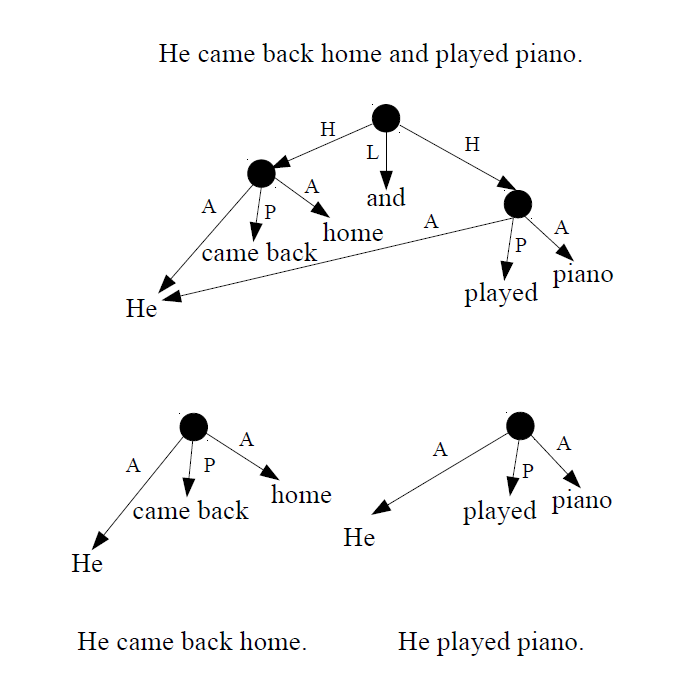
\includegraphics[width=1.2\textwidth,height=48mm]{ucca_simplification}  
    \end{minipage}
}
\end{frame}


\begin{frame}
\frametitle{Graph Structure}
UCCA structures are directed acyclic graphs (DAGs) with labeled edges. \\
Text tokens are terminals, complex units are {\color{blue} non-terminal nodes}. \\
\onslide<2->{
  Phrases may be {\color{red} discontinuous}.
}
\onslide<3->{
  \textit{Remote edges} enable {\color{orange} reentrancy}. \\
}

\hspace*{1cm}
\begin{tikzpicture}[level distance=18mm, sibling distance=28mm, ->,
  level 2/.style={sibling distance=12mm},
  level 3/.style={sibling distance=18mm},
  edge from parent/.append style={nodes={font=\scriptsize}}]
  \tikzstyle{word} = [font=\rmfamily,color=black]
    \node (ROOT) [fill=blue, circle] {}
      child {node (They) [word] {They} edge from parent node[left] {A}}
      child {node [word] {thought} edge from parent node[left] {P}}
      child {node (abouttakingashortbreak) [fill=blue, circle] {}
      {
        child {node [word] {about} edge from parent node[left] {R}}
        child {node (takingabreak) [fill=blue, circle] {}
        {
          child {node [word] {taking} edge from parent node[above] {F}}
          child {node [word] {a} edge from parent node[right] {F}}
          child {node [word] (short) {short} edge from parent[draw=none]}
          child {node [word] {break} edge from parent node[right] {C}}
        } edge from parent node[right] {P} }
      } edge from parent node[right] {A} }
      ;
    \draw[bend left,dashed,->,visible on=<-2>] (abouttakingashortbreak) to node [auto] {\scriptsize A} (They);
    \draw[bend left,dashed,->,orange,very thick,visible on=<3->] (abouttakingashortbreak) to node [auto] {\scriptsize A} (They);
    \draw[bend left,->,visible on=<1>,visible on=<3->] (abouttakingashortbreak) to node [auto] {\scriptsize D} (short);
    \draw[bend left,->,red,very thick,visible on=<2>] (abouttakingashortbreak) to node [auto] {\scriptsize D} (short);
    \node[visible on=<3->] at (6,-.4) {\Large ----- primary edge};
    \node[visible on=<3->] at (6,-1.4) {\Large - - - remote edge};
\end{tikzpicture}

\onslide<2->{
  \vspace{-26mm}
  \begin{adjustbox}{margin=1pt,frame,scale=.9}
    \begin{tabular}{c>{\small\it}l}
        P & Process \\
        A & Participant \\
        C & Center \\
        D & Adverbial \\
        R & Relator \\
        F & Function
    \end{tabular}
  \end{adjustbox}
}
\end{frame}


\begin{frame}
\frametitle{Structural Properties}
\noindent
\centering
\begin{minipage}{.5\linewidth}{\centering
(1) {\color{blue} non-terminal nodes}

\scalebox{.8}{
  \begin{tikzpicture}[level distance=12mm, sibling distance=16mm, ->,
      every node/.append style={midway},
      edge from parent/.append style={nodes={font=\scriptsize}}]
    \node (ROOT) [fill=blue, circle] {}
      child {node [fill=blue, circle] {}
      {
        child {node {John} edge from parent node[left] {C}}
        child {node {and} edge from parent node[left] {N}}
        child {node {Mary} edge from parent node[right] {C}}
      } edge from parent node[left] {A} }
      child {node {went} edge from parent node[left] {P}}
      child {node {home} edge from parent node[right] {A}}
      ;
  \end{tikzpicture}
  }}
\end{minipage}
\hfill
\begin{minipage}{.48\linewidth}{\centering
(2) {\color{red} discontinuity}

\scalebox{.8}{
  \begin{tikzpicture}[level distance=12mm, sibling distance=2cm, ->,
      every node/.append style={midway},
      edge from parent/.append style={nodes={font=\scriptsize}}]
    \node (ROOT) [fill=black, circle] {}
      child {node {John} edge from parent node[left] {A}}
      child {node [fill=black, circle] {}
      {
      	child {node {gave} edge from parent node[left] {C}}
      	child {node (everything) {everything} edge from parent[white]}
      	child {node {up} edge from parent node[right] {C}}
      } edge from parent node[right] {P} }
      ;
    \draw[bend right,->,red,very thick] (ROOT) to[out=-20, in=180] node [left] {\scriptsize A} (everything);
  \end{tikzpicture}
  }}
\end{minipage}

\vfill
(3) {\color{orange} reentrancy}

\scalebox{.8}{
\begin{tikzpicture}[level distance=14mm, sibling distance=17mm, ->,
    edge from parent/.append style={nodes={font=\scriptsize}}]
    \node (ROOT) [fill=black, circle] {}
      child {node (After) {After} edge from parent node[left] {L\;}}
      child {node (graduation) [fill=black, circle] {}
      {
        child {node {graduation} edge from parent node[left] {P}}
      } edge from parent node[left] {H} }
      child {node {,} edge from parent node[right] {U}}
      child {node (moved) [fill=black, circle] {}
      {
        child {node (John) {John} edge from parent node[left] {A}}
        child {node {moved} edge from parent node[left] {P}}
        child {node [fill=black, circle] {}
        {
          child {node {to} edge from parent node[left] {R}}
          child {node {Copenhagen} edge from parent node[right] {C}}
        } edge from parent node[right] {A} }
      } edge from parent node[right] {H} }
      ;
    \draw[dashed,->,orange,very thick] (graduation) to node [auto] {\scriptsize A} (John);
\end{tikzpicture}}
\end{frame}


\begin{frame}
\frametitle{UCCA Data}
\begin{itemize}
 \item English Wikipedia articles (Wiki).
 \item English-French-German parallel corpus from \\ \textit{Twenty Thousand Leagues Under the Sea} (20K).
 \item Reviews from the English Web Treebank (EWT).
\end{itemize}

\vfill
\begin{center}
  \begin{minipage}{.3\textwidth}
\includegraphics[width=\textwidth]{wikipedia.png}\end{minipage}
  \begin{minipage}{.3\textwidth}
\includegraphics[width=\textwidth]{squid.jpg}\end{minipage}
  
  
\includegraphics[width=.3\textwidth]{five-stars.png}
\end{center}
\end{frame}


\begin{frame}
\frametitle{Data Statistics}
\centering
\def\arraystretch{1.5}
\begin{tabular}{l|r|rrr|r}
    & \multicolumn{1}{c|}{Wiki} & \multicolumn{3}{c|}{20K} & \multicolumn{1}{c}{EWT} \\
    & \multicolumn{1}{c|}{en} & \multicolumn{1}{c}{en} & \multicolumn{1}{c}{fr} & \multicolumn{1}{c|}{de} & \multicolumn{1}{c}{en} \\
    \hline
    \# sentences&5,141&492&492&6,514&3,520 \\
    \# tokens&158,739&12,638&13,021&144,529&51,042 \\
    \hline
    \# {\color{blue} non-terminal nodes}&62,002&4,699&5,110&51,934&18,156 \\
    \% {\color{red}discontinuous}&1.71&3.19&4.64&8.87&3.87 \\
    \% {\color{orange}reentrant}&1.84&0.89&0.65&0.31&0.83 \\
    \hline
    \# edges&208,937&16,803&17,520&187,533&60,739 \\
    \% primary&97.40&96.79&97.02&97.32&97.32 \\
    \% remote&2.60&3.21&2.98&2.68&2.68
\end{tabular}
\end{frame}



\section{Transition-based UCCA Parser (ACL'17)}

\begin{frame}
\frametitle{TUPA: Transition-based UCCA Parser}

Parses text $w_1 \ldots w_n$ to graph $G$ incrementally by applying transitions to the parser state,
consisting of: stack, buffer and constructed graph.

\pause
\vfill
Initial state:
\scalebox{.9}{
\begin{tikzpicture}[xscale=1.4,every node/.append style={font=\rmfamily,
                    anchor=west,text height=.6ex,text depth=0}, circle]
    \draw[xstep=1,ystep=.5,color=gray] (-.01,0) grid (1,.5);
    \node[style={font=\sffamily}] at (-.1,.8) {stack};
    \node[fill=black] at (.3,.25) {};
    \draw[xstep=1,ystep=.5,color=gray] (2,0) grid (9,.5);
    \node[style={font=\sffamily}] at (8,.8) {buffer};
    \node at (2,.2) {\small They};
    \node at (3,.2) {\small thought};
    \node at (4,.2) {\small about};
    \node at (5,.2) {\small taking};
    \node at (6,.2) {\small a};
    \node at (7,.2) {\small short};
    \node at (8,.2) {\small break};
\end{tikzpicture}}

\vfill
\pause
\parser{} transitions:

\{\textsc{Shift, Reduce, {\color{blue}Node$_X$}, Left-Edge$_X$, Right-Edge$_X$,}\\
\hspace{5mm}\textsc{{\color{orange}Left-Remote$_X$}, {\color{orange}Right-Remote$_X$}, {\color{red}Swap}, Finish}\}

\vfill
These transition enable {\color{blue}non-terminal nodes}, {\color{orange}reentrancy} and {\color{red}discontinuity}.
\end{frame}

\begin{frame}
\frametitle{Example: TUPA Transition Sequence}
\begin{minipage}[t][8mm][t]{\textwidth}
    $\Rightarrow$\textsc{
        \only<1>{Shift}\only<2>{Right-Edge$_A$}\only<3>{Shift}\only<4>{Swap}\only<5>{Right-Edge$_P$}\only<6>{Reduce}\only<7>{Shift}\only<8>{Shift}\only<9>{Node$_R$}\only<10>{Reduce}\only<11>{Shift}\only<12>{Left-Remote$_A$}\only<13>{Shift}\only<14>{Node$_C$}\only<15>{Reduce}\only<16>{Shift}\only<17>{Right-Edge$_P$}\only<18>{Shift}\only<19>{Right-Edge$_F$}\only<20>{Reduce}\only<21>{Shift}\only<22>{Swap}\only<23>{Right-Edge$_D$}\only<24>{Reduce}\only<25>{Swap}\only<26>{Right-Edge$_A$}\only<27>{Reduce}\only<28>{Reduce}\only<29>{Shift}\only<30>{Reduce}\only<31>{Shift}\only<32>{Right-Edge$_C$}\only<33>{Finish}
    }
\end{minipage}

\vfill

\scalebox{.9}{
\begin{tikzpicture}[xscale=1.4,every node/.append style={font=\rmfamily,
                    anchor=west,text height=.6ex,text depth=0}]
    \begin{scope}[style={font=\sffamily}]
      \node at (-.1,.8) {stack};
      \node at (8,  .8) {buffer};
    \end{scope}
    \begin{scope}[xstep=1,ystep=.5,color=red,line width=1pt]
      \only<31>    \draw (-.01,0) grid (1,.5);
      \only<1,7>   \draw (.99, 0) grid (2,.5);
      \only<2,5,26>\draw (-.01,0) grid (2,.5);
      \only<3,8,11>\draw (1.99,0) grid (3,.5);
      \only<13,16> \draw (2.99,0) grid (4,.5);
      \only<18,21> \draw (3.99,0) grid (5,.5);
      \only<17>    \draw (1.99,0) grid (4,.5);
      \only<19>    \draw (2.99,0) grid (5,.5);
      \only<4>     \draw (3,   0) grid (4,.5);
      \only<9>     \draw (4,   0) grid (5,.5);
      \only<14>    \draw (5,   0) grid (6,.5);
      \only<22>    \draw (7,   0) grid (8,.5);
      \only<25>    \draw (6,   0) grid (7,.5);
      \only<23>    \draw (1.99,0) grid (4,.5);
      \only<32>    \draw (-.01,0) grid (2,.5);
      \only<12>    \draw (.99, 0) grid (3,.5);
    \end{scope}
    \begin{scope}[xstep=1,ystep=.5,color=gray]
      \only<6,27,29,31->         \draw (-.01,0) grid (1, .5);
      \only<-2,4-5,7,10,25-26,33>\draw (-.01,0) grid (2, .5);
      \only<3,8-9,11-12,15,24>   \draw (-.01,0) grid (3, .5);
      \only<13-14,16-17,20,22-23>\draw (-.01,0) grid (4, .5);
      \only<18-19,21>            \draw (-.01,0) grid (5, .5);
      \only<-2,4-6>              \draw (3,   0) grid (9,.5);
      \only<3,5-7,9-10>          \draw (4,   0) grid (9,.5);
      \only<8,11-12,14-15>       \draw (5,   0) grid (9,.5);
      \only<13,16-17,25-28>      \draw (6,   0) grid (9,.5);
      \only<18-20,22-24,29-30>   \draw (7,   0) grid (9,.5);
      \only<21,31>               \draw (8,   0) grid (9,.5);
    \end{scope}
    \begin{scope}[xstep=.1,ystep=.5,color=gray]
      \only<28,30> \draw (-.01,0) grid (.1,.5);
      \only<32->   \draw (8.89,0) grid (9.01,.5);
    \end{scope}
    \only<-27>      \node[fill=black, circle] at (.3, .25) {};
    \only<25-26>    \node[fill=blue,  circle] at (1.3,.25) {};
    \only<11-24>    \node[fill=blue,  circle] at (2.3,.25) {};
    \only<31->      \node[fill=red,   circle] at (.3, .25) {};
    \only<16-21>    \node[fill=red,   circle] at (3.3,.25) {};
    \only<9-10>     \node[fill=blue,  circle] at (4.3,.25) {};
    \only<14-15>    \node[fill=red,   circle] at (5.3,.25) {};
    \only<22-30>    \node[fill=red,   circle] at (7.3,.25) {};
    \only<29>       \node at (0,.2) {\small They};
    \only<1-3,7-24> \node at (1,.2) {\small They};
    \only<4-5>      \node at (1,.2) {\small thought};
    \only<3>        \node at (2,.2) {\small thought};
    \only<8-9>      \node at (2,.2) {\small about};
    \only<13-14>    \node at (3,.2) {\small taking};
    \only<18-19>    \node at (4,.2) {\small a};
    \only<21>       \node at (4,.2) {\small short};
    \only<22-23>    \node at (3,.2) {\small short};
    \only<32->      \node at (1,.2) {\small break};
    \only<4-6>      \node at (3,.2) {\small They};
    \only<25-28>    \node at (6,.2) {\small They};
    \only<-2>       \node at (3,.2) {\small thought};
    \only<-7>       \node at (4,.2) {\small about};
    \only<-12>      \node at (5,.2) {\small taking};
    \only<-17>      \node at (6,.2) {\small a};
    \only<-20>      \node at (7,.2) {\small short};
    \only<-31>      \node at (8,.2) {\small break};
\end{tikzpicture}}
\vfill
\fbox{
\begin{tikzpicture}[level distance=14mm, sibling distance=26mm, ->,
    every node/.append style={font=\rmfamily},
    edge from parent/.append style={nodes={font=\scriptsize}},
    edge from parent path={(\tikzparentnode.center) -- (\tikzchildnode.north)}]
    \node[anchor=west,style={font=\sffamily}] at (0,0) {graph};
    \node(ROOT)[fill=black, circle, visible on=<1->] at (3,0) {}
      child [visible on=<2->,alt=<2>{draw=red}{}] {node (They) {They} edge from parent node [left] {A}}
      child [visible on=<5->,alt=<5>{draw=red}{}] {node (thought) {thought} edge from parent node [left] {P}}
      child [visible on=<9->] {node (abouttakingashortbreak) [fill=blue, circle] {}
      {
        child [visible on=<9->,alt=<9>{draw=red}{}] {node (to) {about} edge from parent node [right] {R}}
        child [visible on=<14->] {node (takingabreak) [fill=red, circle] {}
        {
          child [visible on=<14->] {node (take) {taking} edge from parent node [above] {F}}
          child [visible on=<19->,alt=<19>{draw=red}{}] {node (a) {a} edge from parent node [right] {F}}
          child [visible on=<23->,alt=<23>{draw=red}{}] {node (short) {short} edge from parent [draw=none]}
          child [visible on=<32->,alt=<32>{draw=red}{}] {node (break) {break} edge from parent node [above] {C}}
        } edge from parent [draw=none]}
      } edge from parent [draw=none]}
      ;
    \draw[visible on=<17->,alt=<17>{draw=red}{}] (abouttakingashortbreak) to node [left] {\scriptsize P} (takingabreak);
    \draw[visible on=<26->,alt=<26>{draw=red}{}] (ROOT) to node [left] {\scriptsize A} (abouttakingashortbreak);
    \draw[bend left,dashed, visible on=<12->,alt=<12>{draw=red}{}] (abouttakingashortbreak) to node [auto] {\scriptsize A} (They);
    \draw[bend left, visible on=<23->,alt=<23>{draw=red}{}] (abouttakingashortbreak) to node [auto] {\scriptsize D} (short);
\end{tikzpicture}}
\end{frame}

\begin{frame}
\frametitle{Training}
An \textit{oracle} provides the transition sequence given the correct graph:

\vfill
\centering
\scalebox{.8}{
\begin{tikzpicture}[level distance=15mm, sibling distance=2cm, ->,
    every node/.append style={font=\rmfamily},
    edge from parent/.append style={nodes={font=\scriptsize}},
    edge from parent path={(\tikzparentnode.center) -- (\tikzchildnode.north)}]
    \node(ROOT)[fill=black, circle] at (3,0) {}
      child {node (They) {They} edge from parent node [left] {A}}
      child {node (thought) {thought} edge from parent node [left] {P}}
      child {node (abouttakingashortbreak) [fill=blue, circle] {} 
      { 
        child {node (to) {about} edge from parent node [right] {R}}
        child {node (takingabreak) [fill=red, circle] {}
        {
          child {node (take) {taking} edge from parent node [above] {F}}      
          child {node (a) {a} edge from parent node [right] {F}} 
          child {node (short) {short} edge from parent [draw=none]}
          child {node (break) {break} edge from parent node [above] {C}}  
        } edge from parent [draw=none]}
      } edge from parent [draw=none]}
      ;
    \draw(abouttakingashortbreak) to node [left] {\scriptsize P} (takingabreak); 
    \draw(ROOT) to node [left] {\scriptsize A} (abouttakingashortbreak);
    \draw[bend left,dashed] (abouttakingashortbreak) to node [auto] {\scriptsize A} (They);
    \draw[bend left] (abouttakingashortbreak) to node [auto] {\scriptsize D} (short);
\end{tikzpicture}}
\[\Downarrow\]
\begin{flushleft}
\footnotesize
\textsc{Shift}, \textsc{Right-Edge$_A$}, \textsc{Shift}, \textsc{Swap}, \textsc{Right-Edge$_P$}, \textsc{Reduce}, \textsc{Shift}, \textsc{Shift}, \textsc{Node$_R$}, \textsc{Reduce}, \textsc{Left-Remote$_A$}, \textsc{Shift}, \textsc{Shift}, \textsc{Node$_C$}, \textsc{Reduce}, \textsc{Shift}, \textsc{Right-Edge$_P$}, \textsc{Shift}, \textsc{Right-Edge$_F$}, \textsc{Reduce}, \textsc{Shift}, \textsc{Swap}, \textsc{Right-Edge$_D$}, \textsc{Reduce}, \textsc{Swap}, \textsc{Right-Edge$_A$}, \textsc{Reduce}, \textsc{Reduce}, \textsc{Shift}, \textsc{Reduce}, \textsc{Shift}, \textsc{Right-Edge$_C$}, \textsc{Finish}
\end{flushleft}
\end{frame}

\begin{frame}
\only<-5>{
\frametitle{\parser{} Model}
Learns to greedily predict transition based on current state.

Experimenting with three classifiers:
\vspace{5mm}

    \begin{tabular}{ll}
    \textbf{Sparse} & Perceptron with sparse features. \\
    \textbf{MLP} & Embeddings + MLP. \\
    \textbf{BiLSTM} & Embeddings + \only<2->{\textbf}{bidirectional RNN} + MLP.
    \end{tabular}
}
\only<2-5>{\vspace{-4cm}}

\only<1>{

\vspace{1cm}

Features include:

\{words, POS, syntactic dependencies, existing edge labels\} \\
from the stack and buffer + parents, children, grandchildren.

\vspace{5mm}
\begin{tikzpicture}
    \draw[xstep=1cm,ystep=5mm,color=gray] (-.01,0) grid (4,.5);
    \draw[xstep=1cm,ystep=5mm,color=gray] (5,0) grid (10,.5);
    \node[anchor=west] at (-.1,1) {stack};
    \node[anchor=west] at (8.9,1) {buffer};
    \foreach \i in {0.5,8.5,9.5} {
        \node[fill=gray, circle] at (\i,.25) {};
    }
    \foreach \i in {1.5,2.5,3.5,5.5,6.5,7.5} {
        \node[fill=black, circle] at (\i,.25) {};
    }
\end{tikzpicture}
}
\centering
\onslide<6>{
\fbox{\scalebox{.9}{
\begin{minipage}{.6\textwidth}
\begin{tikzpicture}[xscale=1.3,every node/.append style={font=\rmfamily}]
    \node[anchor=west,style={font=\sffamily}] at (-1,.25){stack};
    \draw[xstep=1,ystep=.5,color=gray] (-.01,0) grid (4,.5);
    \node[fill=black, circle] at (.5,.25) {};
    \node[fill=blue, circle] at (2.5,.25) {};
    \node[anchor=west] at (1,.25) {\small They};
    \node[anchor=west] at (3,.25) {\small taking};
\end{tikzpicture}

\vspace{1cm}
\begin{tikzpicture}[xscale=1.3,every node/.append style={font=\rmfamily}]
    \node[anchor=west,style={font=\sffamily}] at (-1,.25){buffer};
    \draw[xstep=1,ystep=.5,color=gray] (-.01,0) grid (4,.5);
    \node[fill=red, circle] at (.5,.25) {};
    \node[anchor=west] at (1,.25) {\small a};
    \node[anchor=west] at (2,.25) {\small short};
    \node[anchor=west] at (3,.25) {\small break};
\end{tikzpicture}
\end{minipage}
\begin{minipage}{.4\textwidth}
\scalebox{.8}{
\begin{tikzpicture}[xscale=1.5,level distance=1cm, sibling distance=12mm, ->,
    every node/.append style={font=\rmfamily,
                    anchor=west,text height=.6ex,text depth=0},
    edge from parent/.append style={nodes={font=\scriptsize}},
    edge from parent path={(\tikzparentnode.center) -- (\tikzchildnode.north)}]
    \node[anchor=west,style={font=\sffamily}] at (3,0) {graph};
    \draw[color=gray] (.2,.3) rectangle (3.9,-3.2);
    \node(ROOT)[fill=black, circle, visible on=<2->] at (1.2,0) {}
      child {node (They) {They} edge from parent node [left] {A}}
      child {node {thought} edge from parent node [left] {P}}
      child {node (abouttakingashortbreak) [fill=blue, circle] {}
      {
        child {node {about} edge from parent node [left] {R}}
        child {node (takingabreak) [fill=red, circle] {}
        {
          child {node {taking} edge from parent node [above] {F}}
          child [opacity=0] {node {a} edge from parent node [right] {F}}
          child [opacity=0] {node (short) {short} edge from parent [draw=none]}
          child [opacity=0] {node {break} edge from parent node [right] {C}}
        } edge from parent [draw=none]}
      } edge from parent [draw=none]}
      ;
\end{tikzpicture}
}
\end{minipage}
}}}
\onslide<2->{
\scalebox{.65}{
\begin{tikzpicture}[->,every node/.append style={anchor=north,text height=2ex,text depth=0}]
    \tiny
    \tikzstyle{main}=[circle, minimum size=7mm, draw=black!80, node distance=12mm]
    \foreach \i/\word in {1/{They},3/{thought},5/{about},7/{taking},9/{a},11/{short},13/{break}} {
        \onslide<2->\node (x\i) at (\i,-1.3) {\Large\textrm\word};
        \onslide<2->\node[main, fill=white!100] (h\i) at (\i,0) {LSTM};
        \onslide<2->\path (x\i) edge (h\i);
        \onslide<3->\node[main, fill=white!100] (i\i) at (\i.5,.8) {LSTM};
        \onslide<3->\path (x\i) edge [bend right] (i\i);
        \onslide<4->\node[main, fill=white!100] (l\i) at (\i.5,2.3) {LSTM};
        \onslide<4->\path (h\i) edge [bend left] (l\i);
        \onslide<4->\path (i\i) edge (l\i);
        \onslide<5->\node[main, fill=white!100] (k\i) at (\i,3.1) {LSTM};
        \onslide<5->\path (i\i) edge [bend left] (k\i);
        \onslide<5->\path (h\i) edge [bend left] (k\i);
    }
    \foreach \current/\next in {1/3,3/5,5/7,7/9,9/11,11/13} {
        \onslide<2->\path (h\current) edge (h\next);
        \onslide<3->\path (i\next) edge (i\current);
        \onslide<4->\path (l\current) edge (l\next);
        \onslide<5->\path (k\next) edge (k\current);
    }
    \onslide<6>\node[main, fill=white!100] (mlp) at (7,4.6) {MLP};
    \onslide<6>\foreach \i in {1,5,7,9} {
        \path (l\i) edge (mlp);
        \path (k\i) edge (mlp);
    }
    \coordinate (state) at (10.5,6.5);
    \onslide<6>\path (state) edge [bend left] (mlp);
    \onslide<6>\node (transition) at (7,5.8) {\large\textsc{Node}$_C$};
    \onslide<6>\path (mlp) edge (transition);
\end{tikzpicture}
}
}
\end{frame}

\begin{frame}
\frametitle{Comparing to Existing Methods}
Using conversion-based approximation as baseline, \\
with bi-lexical DAG parsers and transition-based tree parsers.

\vfill
\begin{center}
    \begin{dependency}
    \begin{deptext}[column sep=1.5em,ampersand replacement=\^,font=\rmfamily]
	They \^ thought \^ about \^ taking \^ a \^ short \^ break \\
    \end{deptext}
    \depedge{2}{1}{A}
    \depedge[dashed,edge start x offset=6pt,edge end x offset=-6pt,edge unit distance=3.5ex]{7}{1}{A}
    \depedge{7}{3}{R}
    \depedge{7}{4}{F}
    \depedge{7}{5}{F}
    \depedge{7}{6}{D}
    \depedge{2}{7}{A}
    \end{dependency}
    \captionof{figure}{UCCA bi-lexical DAG approximation.}
\end{center}
\end{frame}


\begin{frame}
\frametitle{Bi-lexical Graph Approximation}
\begin{enumerate}
 \item Convert UCCA to bi-lexical DAGs.
 \item Train bi-lexical parsers.
 \item Parse test set.
 \item Convert to UCCA.
 \item Evaluate.
\end{enumerate}

\vspace{-15mm}

\begin{minipage}{.225\textwidth}
  \vspace{1cm}
  \begin{flushright}
    \begin{tikzpicture}[<->]
      \draw [ultra thick,red] (1,1) to[out=180,in=90] (0,0);
    \end{tikzpicture}
  \end{flushright}
\end{minipage}
\begin{minipage}{.7\textwidth}
    \begin{tikzpicture}[level distance=13mm, sibling distance=17mm, ->,
        every circle node/.append style={fill=black},
        edge from parent/.append style={nodes={font=\scriptsize}},
        edge from parent path={(\tikzparentnode.center) -- (\tikzchildnode.north)}]
      \tikzstyle{word} = [font=\rmfamily,color=black]
      \node (ROOT) [circle] {}
        child {node (After) [word] {After} edge from parent node[left] {L}}
        child {node (graduation) [circle] {}
        {
          child {node [word] {graduation} edge from parent node[left] {P}}
        } edge from parent node[left] {H} }
        child {node [word] {,} edge from parent node[right] {U}}
        child {node (moved) [circle] {}
        {
          child {node (John) [word] {John} edge from parent node[left] {A}}
          child {node [word] {moved} edge from parent node[left] {P}}
          child {node [circle] {}
          {
            child {node [word] {to} edge from parent node[left] {R}}
            child {node [word] {Copenhagen} edge from parent node[right] {C}}
          } edge from parent node[right] {A} }
        } edge from parent node[right] {H} }
        ;
      \draw[dashed,->] (graduation) to node [auto] {\scriptsize A} (John);
    \end{tikzpicture}
\end{minipage}

\vspace{-14mm}
\begin{flushleft}
    \begin{dependency}
    \begin{deptext}[column sep=.7em,ampersand replacement=\^,font=\rmfamily]
	After \^ graduation \^ , \^ John \^ moved \^ to \^ Copenhagen \\
    \end{deptext}
    \depedge{2}{1}{L}
    \depedge{2}{3}{U}
    \depedge[dashed]{2}{4}{A}
    \depedge{5}{4}{A}
    \depedge{2}{5}{H}
    \depedge{7}{6}{R}
    \depedge{5}{7}{A}
    \end{dependency}
\end{flushleft}
\end{frame}


\begin{frame}
\frametitle{Evaluation}
\begin{adjustbox}{frame,scale=.75,center}
    \begin{tikzpicture}[level distance=12mm, sibling distance=15mm, ->,
        every circle node/.append style={fill=black},
        edge from parent/.append style={nodes={font=\scriptsize}},
        edge from parent path={(\tikzparentnode.center) -- (\tikzchildnode.north)}]
      \tikzstyle{word} = [font=\rmfamily,color=black]
      \node at (0,.7) {True (human-annotated) graph};
      \node (ROOT) at (0,0) [circle] {}
        child {node (After) [word] {After} edge from parent node[left] {L}}
        child {node (graduation) [circle] {}
        {
          child {node [word] {graduation} edge from parent node[left] {P}}
        } edge from parent node[left] {H} }
        child {node [word] {,} edge from parent node[right] {U}}
        child {node (moved) [circle] {}
        {
          child {node (John) [word] {John} edge from parent node[left] {A}}
          child {node [word] {moved} edge from parent node[left] {P}}
          child {node [circle] {}
          {
            child {node [word] {to} edge from parent node[left] {R}}
            child {node [word] {Copenhagen} edge from parent node[right] {C}}
          } edge from parent node[right] {A} }
        } edge from parent node[right] {H} }
        ;
      \draw[dashed,->] (graduation) to node [auto] {\scriptsize A} (John);
      \node at (8,.7) {Automatically predicted graph for the same text};
      \node (ROOT_) at (7,0) [circle] {}
        child {node (After_) [word] {After} edge from parent node[left] {L}}
        child {node (graduation_) [circle] {}
        {
          child[alt=<2>{red}{}] {node [word] {graduation} edge from parent node[left] {S}}
        } edge from parent node[left] {H} }
        child {node [word] {,} edge from parent node[right] {U}}
        child {node (moved) [circle,xshift=3mm,yshift=-7mm] {}
        {
          child {node (John_) [word] {John} edge from parent node[left] {A}}
          child {node [word] {moved} edge from parent node[left] {P}}
          child[alt=<2>{red}{}] {node [word] {to} edge from parent node[left] {F}}
          child[alt=<2>{red}{}] {node (Copenhagen_) [word] {Copenhagen} edge from parent node[right] {A}}
        } edge from parent node[right] {H} }
        ;
      \draw[dashed,->] (graduation_) to node [auto] {\scriptsize A} (John_);
      \draw[bend left,dashed,->,alt=<2>{red}{}] (graduation_) to[in=90] node [auto] {\scriptsize A} (Copenhagen_);
    \end{tikzpicture}
\end{adjustbox}
\vfill

\begin{enumerate}
  \item Match primary edges between the graphs by terminal yield and label.
  \item Calculate \textbf{precision, recall and F1} scores.
  \item Repeat for remote edges.
\end{enumerate}

\pause
\vfill
\begin{adjustbox}{center}
    \begin{tabular}{c|c|c}
        \multicolumn{3}{l}{Primary} \\
        \textbf{P} & \textbf{R} & \textbf{F1} \\ \hline
        $\frac69=67\%$ & $\frac6{10}=60\%$ & 64\%
    \end{tabular}
    \hspace{1cm}
    \begin{tabular}{c|c|c}
        \multicolumn{3}{l}{Remote} \\
        \textbf{P} & \textbf{R} & \textbf{F1} \\ \hline
        $\frac12=50\%$ & $\frac11=100\%$ & 67\%
    \end{tabular}
\end{adjustbox}
\end{frame}


\begin{frame}
\frametitle{Results}
\onslide<1>{
  \parser{BiLSTM} outperforms all other methods on the English Wiki test set:
}
\onslide<2>{
  \ldots and also on the \textbf{out-of-domain} English 20K:
}
\begin{center}
    \begin{tabular}{l|c|c}
        & \multicolumn{2}{c}{English Wiki} \\
        & \tiny Primary & \tiny Remote \\
        & \scriptsize \textbf{F1} & \scriptsize \textbf{F1} \\
        \hline
        \scriptsize \parser{} & \\
        Sparse
        & 64.1 & 16 \\
        MLP
        & 64.9 & 16.9 \\
        BiLSTM
        & \textbf{73.3} & \textbf{47.2} \\
        \hline
        \tiny Baselines & \\
    	\scriptsize DAGParser
        & 58.6 & 1 \\
    	\scriptsize TurboParser
        & 51.2 & 3.7 \\
    	\scriptsize MaltParser
        & 60.2 \\
    	\scriptsize StackLSTM
        & 69.9 \\
        \scriptsize UPARSE
        & 61.1
    \end{tabular}
    \hspace{-2mm}
    \onslide<2->{
    \begin{tabular}{|c|c}
        \multicolumn{2}{|c}{English 20K} \\
        \tiny Primary & \tiny Remote \\
        \scriptsize \textbf{F1} & \scriptsize \textbf{F1} \\
        \hline\\
        59.8 & 11.5 \\
        62.5 & 9.7 \\
        \textbf{68.2} & \textbf{23.7} \\
        \hline\\
        53.4 \\
        43.1 & 0.8 \\
        55.3 \\
        63.5 \\
        52.8
    \end{tabular}
    \hspace{-2mm}
    }
    \onslide<3->{
    \begin{tabular}{|c|c}
        \multicolumn{2}{|c}{French 20K} \\
        \tiny Primary & \tiny Remote \\
        \scriptsize \textbf{F1} & \scriptsize \textbf{F1} \\
        \hline\\\\\\
        67.6 & 13.9 \\
        \hline\\\\\\\\\\\\
    \end{tabular}
    \hspace{-2mm}
    \begin{tabular}{|c|c}
        \multicolumn{2}{|c}{German 20K} \\
        \tiny Primary & \tiny Remote \\
        \scriptsize \textbf{F1} & \scriptsize \textbf{F1} \\
        \hline\\\\\\
        72.5 & 27.1 \\
        \hline\\\\\\\\\\\\
    \end{tabular}
    }
\end{center}
\end{frame}

\begin{frame}
\frametitle{Interim Summary}
\begin{itemize}
 \item UCCA's semantic distinctions require a graph structure including {\color{blue}non-terminals}, {\color{orange}reentrancy} and {\color{red}discontinuity}.
 \item \parser{} is an accurate transition-based UCCA parser,
 	and the first to support UCCA and any DAG over the text tokens.
 \item Outperforms strong conversion-based baselines.
\end{itemize}

\pause
\vfill

Up next:

\begin{itemize}
 \item Parsing other semantic representations.
 \item Comparing representations through conversion.
\end{itemize}
\end{frame}



\section{Multitask Parsing across Semantic Representations (ACL'18)}


\begin{frame}
    \frametitle{Semantic Representations}

      \begin{flushright}
        \scalebox{.6}{
\begin{tikzpicture}[level distance=2cm, sibling distance=25mm, ->, draw=Indigo, alt=<3->{opacity=.3}{}]
    \node[font=\bf\sffamily\Huge,Indigo] at (-3,0) {UCCA};
    \node (ROOT) [fill=Indigo, circle] {}
      child {node (After) {After} edge from parent node[left] {L\;}}
      child {node (graduation) [fill=Indigo, circle] {}
      {
        child {node {graduation} edge from parent node[left] {P}}
      } edge from parent node[left] {H} }
      child {node {,} edge from parent node[right] {U}}
      child {node (moved) [fill=Indigo, circle] {}
      {
        child {node (John) {John} edge from parent node[left] {A}}
        child {node {moved} edge from parent node[left] {P}}
        child {node [fill=Indigo, circle] {}
        {
          child {node {to} edge from parent node[left] {R}}
          child {node {Copenhagen} edge from parent node[left] {C}}
        } edge from parent node[left] {A} }
      } edge from parent node[right] {H} }
      ;
    \draw[dashed,->] (graduation) to node [auto] {\scriptsize A} (John);
\end{tikzpicture}
        }
      \end{flushright}
    
    \vspace{-23mm}
    
    \scalebox{.6}{
\begin{tikzpicture}[alt=<2>{opacity=.3}{},alt=<4->{opacity=.3}{}]
\node[font=\bf\sffamily\Huge,DarkGreen] at (0,6) {AMR};
\graph[layered layout, sibling distance=4cm, layer distance=2cm, nodes={ellipse,draw=DarkGreen}, edges={nodes={sloped}, DarkGreen}]{
a4 Copenhagen[as={Copenhagen}];
a2 John[as={John}];
a1[as={person}];
a0[as={move-01}];
a3[as={city}];
a2[as={name}];
a5[as={after}];
a4[as={name}];
a6[as={graduate-01}];

a1 ->  ["name"' above] a2;
a0 ->  ["ARG0"' above] a1;
a0 ->  ["ARG2"' above] a3;
a0 ->  ["time"' above] a5;
a3 ->  ["name"' above] a4;
a2 ->  ["op1"' above] a2 John;
a5 ->  ["op1"' above] a6;
a4 ->  ["op1"' above] a4 Copenhagen;
};
\draw[->, above, DarkGreen] (a6) to node[sloped] {ARG0} (a1);
\end{tikzpicture}
      }
    \vspace{-15mm}
    
    \begin{flushright}
    \begin{minipage}{.01\textwidth}
      \begin{tikzpicture}[alt=<2-3>{opacity=.3}{}]
        \node[font=\bf\sffamily\Large,DarkRed] {DM};
      \end{tikzpicture}
    \end{minipage}
    \begin{minipage}{.6\textwidth}
        \rmfamily
        \scalebox{.7}{
\begin{dependency}[theme=simple,edge style={-{Latex[length=2mm]}, color=DarkRed}, alt=<2-3>{opacity=.3}{},
            text only label, label style={above, color=DarkRed, font=\bf\ttfamily}, font=\small]
    \begin{deptext}[column sep=1em,ampersand replacement=\^]
	After \^ graduation \^ , \^ John \^ moved \^ to \^ Copenhagen \\
    \end{deptext}
    \deproot{5}{top}
    \depedge{1}{2}{ARG2}
    \depedge{1}{5}{ARG1}
    \depedge{5}{4}{ARG1}
    \depedge{6}{5}{ARG1}
    \depedge{6}{7}{ARG2}
\end{dependency}
    }
    \end{minipage}
    \end{flushright}
\end{frame}


\begin{frame}
\frametitle{Syntactic Representations}
    {\color{DarkBlue}\bf\sffamily\Large UD} (Universal Dependencies)
    
    \begin{center}
    \rmfamily
    \begin{dependency}[text only label, edge style={-{Latex[length=2mm]}, color=DarkBlue},
                       label style={above, color=DarkBlue, font=\bf\ttfamily}, font=\small]
    \begin{deptext}[column sep=.8em,ampersand replacement=\^]
    After \^ graduation \^ , \^ John \^ moved \^ to \^ Copenhagen \\
    \end{deptext}
        \depedge{2}{1}{case}
        \depedge{2}{3}{punct}
        \depedge{5}{4}{nsubj}
        \depedge[edge end x offset=-2pt]{5}{2}{obl}
        \depedge{7}{6}{case}
        \deproot[edge unit distance=2.5ex]{5}{root}
        \depedge{5}{7}{obl}
    \end{dependency}
    \end{center}
\end{frame}


\begin{frame}
    \frametitle{Data}
    \fbox{UCCA training data is scarce}
    \begin{center}
    \begin{minipage}{.15\textwidth}
      (English)
    \end{minipage}
    \begin{minipage}{.7\textwidth}
    \pgfplotstableread[row sep=\\,col sep=&]{
    	corpus & total \\
        \color{DarkBlue} \textbf{UD} & 17062 \\
        \color{DarkRed} \textbf{DM} & 33964 \\
        \color{DarkGreen} \textbf{AMR} & 36521 \\
        \color{Indigo} \textbf{UCCA} & 5141 \\
        }\english
        \begin{tikzpicture}
        \begin{axis}[
        xbar stacked,
        width=10cm,
        height=39mm,
        xmin=0,
        xmax=60000,
        xtick=\empty,
        ytick=data,
        yticklabels from table={\english}{corpus},
        axis x line=none,
        ]
        \addplot [fill=Navy, point meta=explicit symbolic,
        nodes near coords={\pgfmathprintnumber\pgfplotspointmeta~sentences},
        nodes near coords align={anchor=west}] table [x=total,y expr=\coordindex,meta=total] {\english};
        \end{axis}
        \end{tikzpicture}
    \end{minipage}
    \end{center}
    
    \pause
    \vfill
    
    \begin{flushright}
        \fbox{and domains are limited.}
    \end{flushright}
    \begin{center}
    \begin{tabular}{llll}
        \color{Indigo} \textbf{UCCA}  & \color{DarkGreen} \textbf{AMR}  & \color{DarkRed} \textbf{DM}  & \color{NavyBlue} \textbf{UD}  \\
    	Wikipedia & blogs & news & blogs \\ books & news && news \\ & emails && emails \\ & reviews && reviews \\ &&& Q\&A
    \end{tabular}
    \end{center}
\end{frame}


\begin{frame}
\frametitle{Conversion}

\begin{minipage}{.04\textwidth}
\vspace{4mm}
\color{DarkGreen} AMR\\
\vspace{13mm}
\color{DarkRed} DM\\
\vspace{14mm}
\color{DarkBlue} UD
\end{minipage}
\begin{minipage}{.45\textwidth}
  \centering
  \scalebox{.6}{
  \begin{tikzpicture}[->,draw=DarkGreen,
      every node/.append style={sloped,anchor=south,auto=false,font=\tiny},
      level 1/.style={level distance=14mm,sibling distance=26mm},
      level 2/.style={level distance=13mm},
      level 3/.style={level distance=12mm}]
    \node (ROOT) [draw=black,ellipse] {move-01}
      child {node [draw=black,ellipse] {after}
      {
            child {node (graduation) [draw=black,ellipse] {graduate-01} edge from parent node {op1} }
      } edge from parent node {time} }
      child {node (John) [draw=black,ellipse] {person}
      {
        child {node [draw=black,ellipse] {name}
        {
            child {node [draw=black,ellipse] {"John"} edge from parent node {op1} }
        } edge from parent node {name} }
      } edge from parent node {ARG0} }
      child {node [draw=black,ellipse] {city}
      {
        child {node [draw=black,ellipse] {name}
        {
            child {node [draw=black,ellipse] {"Copenhagen"} edge from parent node {op1} }
        } edge from parent node {name} }
      } edge from parent node {ARG2} }
      ;
      \draw (graduation) to node {ARG0} (John);
  \end{tikzpicture}
  }
  
  \vspace{5mm}
  \scalebox{.6}{
    \begin{dependency}[text only label, font=\small, edge style={color=DarkRed},
                       label style={above, color=DarkRed, font=\bf\ttfamily}]
    \begin{deptext}[column sep=.8em,ampersand replacement=\^]
    After \^ graduation \^ , \^ John \^ moved \^ to \^ Copenhagen \\
    \end{deptext}
        \depedge{1}{2}{ARG2}
        \depedge{5}{4}{ARG1}
        \depedge[edge end x offset=-2pt]{1}{5}{ARG1}
        \deproot[edge unit distance=3.5ex]{5}{top}
        \depedge[edge start x offset=-1pt, edge end x offset=3pt]{5}{7}{ARG2}
        \depedge[edge end x offset=5pt]{6}{5}{ARG1}
        \depedge{6}{7}{ARG2}
    \end{dependency}
    }
    
  \vspace{5mm}
  \scalebox{.6}{
    \begin{dependency}[text only label, edge style={color=DarkBlue},
                       label style={above, color=DarkBlue, font=\bf\ttfamily}, font=\small]
    \begin{deptext}[column sep=.8em,ampersand replacement=\^]
    After \^ graduation \^ , \^ John \^ moved \^ to \^ Copenhagen \\
    \end{deptext}
        \depedge{2}{1}{case}
        \depedge{2}{3}{punct}
        \depedge{5}{4}{nsubj}
        \depedge[edge end x offset=-2pt]{5}{2}{obl}
        \depedge{7}{6}{case}
        \deproot[edge unit distance=2.5ex]{5}{root}
        \depedge{5}{7}{obl}
    \end{dependency}
    }

\end{minipage}
\begin{minipage}{.02\textwidth}
\vspace{7mm}
\Rightarrow
\vspace{16mm}
\Rightarrow
\vspace{20mm}
\Rightarrow
\end{minipage}
\begin{minipage}{.45\textwidth}

  \centering
  \scalebox{.6}{
  \begin{tikzpicture}[level distance=16mm, ->,
      every node/.append style={sloped,anchor=south,auto=false,font=\scriptsize},
      level 1/.style={sibling distance=28mm},
      level 2/.style={sibling distance=14mm},
      level 3/.style={sibling distance=12mm},
      edge from parent path={(\tikzparentnode.center) -- (\tikzchildnode.north)}]
    \tikzstyle{word} = [font=\rmfamily,color=black]
    \node (ROOT) [word] {moved}
      child {node [word] {After}
      {
            child {node (graduation) [word] {graduation} edge from parent node {op} }
      } edge from parent node {time} }
      child {node (John) [fill=black,circle] {}
      {
        child {node [word] {John} edge from parent node {name} }
      } edge from parent node {ARG0} }
      child {node [fill=black,circle] {}
      {
        child {node [word] {Copenhagen} edge from parent node {name} }
      } edge from parent node {ARG2} }
      ;
      \draw[dashed] (graduation) to node {ARG0} (John);
  \end{tikzpicture}}

  \vspace{5mm}
  \scalebox{.6}{
  \begin{tikzpicture}[level distance=14mm, ->,
      every node/.append style={sloped,anchor=south,auto=false,font=\scriptsize},
      level 1/.style={sibling distance=29mm,level distance=6mm},
      level 2/.style={sibling distance=16mm,level distance=14mm},
      edge from parent path={(\tikzparentnode.center) -- (\tikzchildnode.north)}]
    \tikzstyle{word} = [font=\rmfamily,color=black]
    \node (ROOT) [fill=black,circle] {}
      child {node (after) [fill=black,circle] {}
      {
        child {node [draw=none] {}
        {
          child {node [word] (after_word) {After{\color{white}g}} edge from parent [draw=none]}
        } edge from parent [draw=none] }
        child {node [draw=none] {}
        {
          child {node [word] (graduation) {graduation ,} edge from parent [draw=none]}
        } edge from parent [draw=none] }
      } edge from parent node {root}}
      child {node [draw=none] {}
      {
        child {node (moved) [fill=black,circle] {}
        {
          child {node [word] {\quad{\color{white}g} John} edge from parent node {ARG1}}
          child {node [word] {moved{\color{white}g}} edge from parent node {head}}
        } edge from parent [draw=none] }
      } edge from parent [draw=none] }
      child {node (to) [fill=black,circle] {}
      {
        child {node [draw=none] {}
        {
            child {node [word] (to_word) {to{\color{white}g}} edge from parent [draw=none]}
          } edge from parent [draw=none] }
          child {node [draw=none] {}
        {
          child {node [word] (Copenhagen) {Copenhagen{\color{white}g}} edge from parent [draw=none]}
        } edge from parent [draw=none] }
      } edge from parent node {root}}
      ;
      \draw (ROOT) to node {top} (moved);
      \draw (after) to node {head} (after_word);
      \draw (after) to node {ARG2} (graduation);
      \draw[dashed] (after) to node {ARG1} (moved);
      \draw[dashed] (to) to node {ARG1} (moved);
      \draw (to) to node {head} (to_word);
      \draw (moved) to node {ARG2} (Copenhagen);
      \draw[dashed] (to) to node {ARG2} (Copenhagen);
  \end{tikzpicture}}

  \vspace{5mm}
  \scalebox{.6}{
  \begin{tikzpicture}[level distance=15mm, ->,
      every node/.append style={sloped,anchor=south,auto=false,font=\scriptsize},
      level 1/.style={sibling distance=16mm},
      level 2/.style={sibling distance=12mm},
      edge from parent path={(\tikzparentnode.center) -- (\tikzchildnode.north)}]
    \tikzstyle{word} = [font=\rmfamily,color=black]
    \node (ROOT) [fill=black,circle] {}
      child {node (after) [fill=black,circle] {}
      {
        child {node [word] {After{\color{white}g}\quad\quad} edge from parent node {case}}
        child {node [word] {\quad graduation\quad\quad} edge from parent node {head}}
      } edge from parent node {obl}}
      child {node {}
      {
        child {node [word] (comma) {\quad,{\color{white}g}} edge from parent [draw=none]}
      } edge from parent [draw=none]}
      child {node {}
      {
        child {node [word] (John) {John{\color{white}g}} edge from parent [draw=none]}
      } edge from parent [draw=none]}
      child {node {}
      {
        child {node [word] (moved) {moved{\color{white}g}} edge from parent [draw=none]}
      } edge from parent [draw=none]}
      child {node (to) [fill=black,circle] {}
      {
          child {node [word] {to{\color{white}g}} edge from parent node {case}}
          child {node [word] {Copenhagen{\color{white}g}} edge from parent node {head}}
      } edge from parent node {obl}}
      ;
      \draw (ROOT) to node {punct} (comma);
      \draw (ROOT) to node {nsubj} (John);
      \draw (ROOT) to node {head} (moved);
  \end{tikzpicture}}

\end{minipage}

\end{frame}


\begin{frame}
    \frametitle{Multitask}
\centering
    \begin{minipage}{.05\pagewidth}
    \scalebox{6}{\{}
    \end{minipage}
    \begin{minipage}{.3\pagewidth}
        \scalebox{.31}{
\begin{tikzpicture}[level distance=2cm, sibling distance=25mm, ->, draw=Indigo,
    edge from parent/.append style={nodes={font=\scriptsize}},
    edge from parent path={(\tikzparentnode.center) -- (\tikzchildnode.north)}]
    \node (ROOT) [fill=Indigo, circle] {}
      child {node (After) {After} edge from parent node[left] {L\;}}
      child {node (graduation) [fill=Indigo, circle] {}
      {
        child {node {graduation} edge from parent node[left] {P}}
      } edge from parent node[left] {H} }
      child {node {,} edge from parent node[right] {U}}
      child {node (moved) [fill=Indigo, circle] {}
      {
        child {node (John) {John} edge from parent node[left] {A}}
        child {node {moved} edge from parent node[left] {P}}
        child {node [fill=Indigo, circle] {}
        {
          child {node {to} edge from parent node[left] {R}}
          child {node {Copenhagen} edge from parent node[left] {C}}
        } edge from parent node[left] {A} }
      } edge from parent node[right] {H} }
      ;
    \draw[dashed,->] (graduation) to node [auto] {\scriptsize A} (John);
\end{tikzpicture}
        }
    \end{minipage}
    \begin{minipage}{.24\pagewidth}
    \scalebox{.3}{
\begin{tikzpicture}
\graph[layered layout, sibling distance=4cm, layer distance=2cm, nodes={ellipse,draw=DarkGreen}, edges={nodes={sloped}, DarkGreen}]{
a4 Copenhagen[as={Copenhagen}];
a2 John[as={John}];
a1[as={person}];
a0[as={move-01}];
a3[as={city}];
a2[as={name}];
a5[as={after}];
a4[as={name}];
a6[as={graduate-01}];

a1 ->  ["name"' above] a2;
a0 ->  ["ARG0"' above] a1;
a0 ->  ["ARG2"' above] a3;
a0 ->  ["time"' above] a5;
a3 ->  ["name"' above] a4;
a2 ->  ["op1"' above] a2 John;
a5 ->  ["op1"' above] a6;
a4 ->  ["op1"' above] a4 Copenhagen;
};
\draw[->, above, DarkGreen] (a6) to node[sloped] {ARG0} (a1);
\end{tikzpicture}
      }
    \end{minipage}
    \begin{minipage}{.22\pagewidth}
        \rmfamily
        \scalebox{.33}{
\begin{dependency}[theme=simple,edge style={-{Latex[length=2mm]}, color=DarkRed},
            text only label, label style={above, color=DarkRed, font=\bf\ttfamily}, font=\small]
    \begin{deptext}[column sep=1.5em,ampersand replacement=\^]
	After \^ graduation \^ , \^ John \^ moved \^ to \^ Copenhagen \\
    \end{deptext}
    \deproot{5}{top}
    \depedge{1}{2}{ARG2}
    \depedge{1}{5}{ARG1}
    \depedge{5}{4}{ARG1}
    \depedge{6}{5}{ARG1}
    \depedge{6}{7}{ARG2}
\end{dependency}
    }
    
        \scalebox{.33}{
    \begin{dependency}[edge style={-{Latex[length=2mm]}, color=DarkBlue},
        text only label, label style={above, color=DarkBlue, font=\bf\ttfamily}, font=\small]
    \begin{deptext}[column sep=1.5em,ampersand replacement=\^, color=DarkBlue]
    After \^ graduation \^ , \^ John \^ moved \^ to \^ Copenhagen \\
    \end{deptext}
        \depedge[edge unit distance=1em]{2}{1}{case}
        \depedge[edge unit distance=1em]{2}{3}{punct}
        \depedge[edge unit distance=1em, edge start x offset=-4mm]{5}{4}{nsubj}
        \depedge[edge unit distance=1em, edge end x offset=-3mm]{5}{2}{obl}
        \depedge[edge unit distance=1em]{7}{6}{case}
        \deproot[edge unit distance=1em]{5}{root}
        \depedge[edge unit distance=1.5em, edge start x offset=1mm]{5}{7}{obl}
    \end{dependency}
    }
    \end{minipage}
    \begin{minipage}{.05\pagewidth}
    \scalebox{6}{\}}
    \end{minipage}
    
    \pause
    \vfill
    
    \begin{center}\scalebox{.3}{\Huge
       \begin{tikzpicture}[-{Latex[length=3mm]},thick]
       \tikzstyle{main}=[rounded rectangle, minimum size=35mm, draw=black!80, node distance=12mm]
       \node[main] (specific) at (0,12) {Task-specific BiLSTM};
       \node[main,color=DarkCyan] (shared) at (22,12) {Shared BiLSTM};
       \foreach \i/\word in {-4/{After},4/{graduation},17/{to},25/{Copenhagen}} {
           \node (x\i) at (\i,3) {\word};
           \node[main, minimum size=16mm, fill=DarkCyan, draw=none] (e\i) at (\i,6) {};
           \path[color=DarkCyan] (x\i) edge (e\i);
           \path (e\i) edge (specific);
           \path[color=DarkCyan] (e\i) edge (shared);
       }
        \node (x4) at (10.5,3) {\ldots};
        \node[main] (mlp) at (10.5,15) {MLP};
        \path (specific) edge (mlp);
        \path[color=DarkCyan] (shared) edge (mlp);
        \node (transition) at (10.5,17.8) {};
        \path (mlp) edge node[right] {} (transition);
       \end{tikzpicture}}
    \end{center}
\end{frame}

\begin{frame}
\frametitle{Results}
\centering
\small
\setlength\tabcolsep{3pt}
\begin{tabular}{lcc}
& \footnotesize \bf Primary F1 & \footnotesize \bf Remote F1 \\
\hline
\multicolumn{3}{l}{\small \bf English (in-domain)} \\
\footnotesize Single
& 73.6 & 51.5 \\
\cline{1-1}
%\small \bf Multitask &&& \\
\footnotesize +AMR
& 73.7 & 49.9 \\
\footnotesize +DM
& 74.8 & \textbf{53.9} \\
\footnotesize +UD
& 74.1 & 50.8 \\
\footnotesize +AMR+DM
& 74.7 & 51.4 \\
\footnotesize +AMR+UD
& 73.8 & 48.5 \\
\footnotesize +DM+UD
& \textbf{74.9} & 51.2 \\
\footnotesize All
& 74.4 & 52
\end{tabular}
\hfill
\begin{tabular}{lcc}
& \footnotesize \bf Primary F1 & \footnotesize \bf Remote F1 \\
\hline
\multicolumn{3}{l}{\small \bf English (out-of-domain)} \\
\footnotesize Single
& 69 & 26.7 \\
\cline{1-1}
%\small \bf Multitask &&& \\
\footnotesize +AMR
& 69.5 & 27.5 \\
\footnotesize +DM
& 70.7 & 25.9 \\
\footnotesize +UD
& 69.7 & 28.7 \\
\footnotesize +AMR+DM
& 70.5 & 27.3 \\
\footnotesize +AMR+UD
& 70 & 29.4 \\
\footnotesize +DM+UD
& 70.6 & 28.4 \\
\footnotesize All
& \textbf{71} & \textbf{29.6}
\end{tabular}
\vfill
\begin{tabular}{lcc}
& \footnotesize \bf Primary F1 & \footnotesize \bf Remote F1 \\
\hline
\multicolumn{3}{l}{\small \bf French (in-domain)} \\
\small Single & 67.6 & 13.9 \\
\small +UD & \textbf{70.1} & 20.3 \\
\hline
\multicolumn{3}{l}{\small \bf German (in-domain)} \\
\small Single & 72.5 & 27.1 \\
\small +UD & \textbf{73.2} & \textbf{35.5}
\end{tabular}
\end{frame}




\section{Content Differences in Syntactic and Semantic Representations}


\begin{frame}
    \frametitle{UCCA}
      \begin{center}
\begin{tikzpicture}[level distance=2cm, sibling distance=25mm, ->, draw=Indigo,
    edge from parent/.append style={nodes={font=\scriptsize}},
    edge from parent path={(\tikzparentnode.center) -- (\tikzchildnode.north)}]
    \node (ROOT) [fill=Indigo, circle] {}
      child {node (After) {After} edge from parent node[left] {L\;}}
      child {node (graduation) [fill=Indigo, circle] {}
      {
        child {node {graduation} edge from parent node[left] {P}}
      } edge from parent node[left] {H} }
      child {node {,} edge from parent node[right] {U}}
      child {node (moved) [fill=Indigo, circle] {}
      {
        child {node (John) {John} edge from parent node[left] {A}}
        child {node {moved} edge from parent node[left] {P}}
        child {node [fill=Indigo, circle] {}
        {
          child {node {to} edge from parent node[left] {R}}
          child {node {Copenhagen} edge from parent node[left] {C}}
        } edge from parent node[left] {A} }
      } edge from parent node[right] {H} }
      ;
    \draw[dashed,->] (graduation) to node [auto] {\scriptsize A} (John);
\end{tikzpicture}
      \end{center}
\end{frame}

\begin{frame}
    \frametitle{UCCA}
\begin{tikzpicture}[level distance=19mm, sibling distance=21mm, ->, draw=Indigo,
  edge from parent/.append style={nodes={font=\scriptsize}},
      edge from parent path={(\tikzparentnode.center) -- (\tikzchildnode.north)}]
  \tikzstyle{word} = [font=\rmfamily,color=black]
    \node (ROOT) [fill=Indigo, circle] {}
      child {node (They) [word] {They} edge from parent node[left] {A}}
      child {node [word] {thought} edge from parent node[left] {D}}
      child {node [word] {about} edge from parent node[left] {R}}
      child {node (takingashortbreak) [fill=Indigo, circle] {}
      {
        child {node [word] {taking} edge from parent node[above] {F}}
        child {node [word] {a} edge from parent node[right] {F}}
        child {node [word] (short) {short} edge from parent[draw=none]}
        child {node [word] {break} edge from parent node[right] {C}}
      } edge from parent node[right] {P} }
      ;
    \draw[bend left,->] (ROOT) to[out=45,in=110] node [auto] {\scriptsize D} (short);
\end{tikzpicture}
\end{frame}


\begin{frame}
\frametitle{UCCA vs. UD}
\centering
  \scalebox{.8}{
    \begin{tikzpicture}[level distance=9mm, sibling distance=28mm, ->, draw=Indigo,
        every circle node/.append style={fill=Indigo},
        edge from parent/.append style={nodes={font=\scriptsize}},
        edge from parent path={(\tikzparentnode.center) -- (\tikzchildnode.north)}]
      \tikzstyle{word} = [font=\rmfamily,color=black]
      \node[color=Indigo] at (-4,0) {UCCA:};
      \node[color=DarkBlue] at (-4,-3) {UD:};
      \node (ROOT) [circle] {}
        child {node (After) [word] {After} edge from parent node[above] {L}}
        child {node (graduation) [circle] {}
        {
          child {node [word] {graduation} edge from parent node[left] {P}}
        } edge from parent node[right] {H} }
        child {node [word] {,} edge from parent node[below] {U}}
        child {node (moved) [circle] {}
        {
          child {node (John) [word] {John} edge from parent node[left] {A}}
          child {node [word] {moved} edge from parent node[left] {P}}
          child {node [circle] {}
          {
            child {node [word] {to} edge from parent node[left] {R}}
            child {node [word] {Copenhagen} edge from parent node[right] {C}}
          } edge from parent node[above] {A} }
        } edge from parent node[right] {H} }
        ;
      \draw[dashed,->] (graduation) to node [above] {\scriptsize A} (John);
    \end{tikzpicture}
    }
    
    \begin{dependency}[text only label, label style={above,font=\tt, color=DarkBlue}, edge style={color=DarkBlue}, font=\small\rmfamily]
    \begin{deptext}[column sep=1.8em,ampersand replacement=\^]
    After \^ graduation \^ , \^ John \^ moved \^ to \^ Copenhagen \\
    \end{deptext}
        \depedge[edge unit distance=1ex]{2}{1}{case}
        \depedge[edge unit distance=1ex]{2}{3}{punct}
        \depedge[edge unit distance=1ex]{5}{4}{nsubj}
        \depedge[edge unit distance=1ex, edge end x offset=-2pt]{5}{2}{obl}
        \depedge[edge unit distance=1ex]{7}{6}{case}
        \deproot[edge unit distance=1.5ex]{5}{root}
        \depedge[edge unit distance=1.5ex]{5}{7}{obl}
    \end{dependency}
    
    \hrulefill
    
  \scalebox{.7}{
  \begin{tikzpicture}[level distance=12mm, ->, draw=DarkBlue,
      every node/.append style={sloped,anchor=south,auto=false,font=\scriptsize\tt,color=DarkBlue},
      level 2/.style={sibling distance=27mm,level distance=9mm},
      level 3/.style={sibling distance=22mm,level distance=14mm},
      edge from parent/.append style={nodes={font=\scriptsize}},
      edge from parent path={(\tikzparentnode.center) -- (\tikzchildnode.north)}]
    \tikzstyle{word} = [font=\rmfamily,color=black]
      \node at (-4.75,0) {\normalsize\sffamily Converted UD:};
    \node [fill=DarkBlue,circle] {}
      child {node (ROOT) [fill=DarkBlue,circle] {}
      {
        child {node (after) [fill=DarkBlue,circle] {}
        {
          child {node [word] {After{\color{white}g}\quad\quad} edge from parent node {case}}
          child {node [word] {\quad graduation\quad\quad} edge from parent node {head}}
        } edge from parent node {obl}}
        child {node {}
        {
          child {node [word] (comma) {\quad,{\color{white}g}} edge from parent [draw=none]}
        } edge from parent [draw=none]}
        child {node {}
        {
          child {node [word] (John) {John{\color{white}g}} edge from parent [draw=none]}
        } edge from parent [draw=none]}
        child {node {}
        {
          child {node [word] (moved) {moved{\color{white}g}} edge from parent [draw=none]}
        } edge from parent [draw=none]}
        child {node (to) [fill=DarkBlue,circle] {}
        {
            child {node [word] {to{\color{white}g}} edge from parent node {case}}
            child {node [word] {Copenhagen{\color{white}g}} edge from parent node {head}}
        } edge from parent node {obl}}
      } edge from parent node {head}}
      ;
      \draw (ROOT) to node {punct} (comma);
      \draw (ROOT) to node {nsubj} (John);
      \draw (ROOT) to node {head} (moved);
  \end{tikzpicture}}
\end{frame}

\begin{frame}
\frametitle{Confusion Matrix}
\vspace{-1cm}
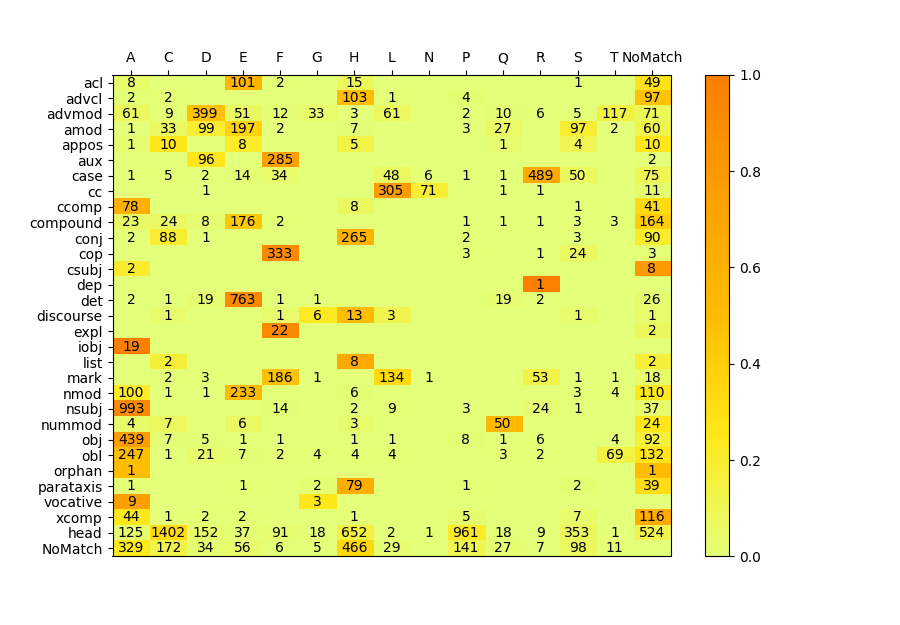
\includegraphics[width=1.15\textwidth]{confusion_matrix.png}
\end{frame}

\begin{frame}
\frametitle{Divergences}
\centering
\begin{tabular}{cc}
\bf UCCA & \bf UD \\\\
Scene/non-Scene & POS-based distinction \\\\
primary/secondary relations, & core/non-core arguments \\
participants & \\\\
more MWEs & less MWEs \\\\
Participant/Elaborator/ & coordination/subordination/ \\
Parallel Scenes & complementation/parataxis
\end{tabular}

\begin{minipage}{.4\textwidth}
  \scalebox{.8}{
    \begin{tikzpicture}[level distance=9mm, sibling distance=14mm, ->, draw=Indigo,
        every circle node/.append style={fill=Indigo},
        edge from parent/.append style={nodes={font=\scriptsize}},
        edge from parent path={(\tikzparentnode.center) -- (\tikzchildnode.north)}]
      \tikzstyle{word} = [font=\rmfamily,color=black]
      \node (ROOT) [circle] {}
        child {node (After) [word] {After} edge from parent node[above] {L}}
        child {node (graduation) [circle] {}
        {
          child {node [word] {graduation} edge from parent node[left] {P}}
        } edge from parent node[right] {H} }
        child {node [word] {,} edge from parent node[below] {U}}
        child {node (moved) [circle] {}
        {
          child {node (John) [word] {John} edge from parent node[left] {A}}
          child {node [word] {moved} edge from parent node[left] {P}}
          child {node [circle] {}
          {
            child {node [word] {to} edge from parent node[left] {R}}
            child {node [word] {Copenhagen} edge from parent node[right] {C}}
          } edge from parent node[above] {A} }
        } edge from parent node[right] {H} }
        ;
      \draw[dashed,->] (graduation) to node [above] {\scriptsize A} (John);
    \end{tikzpicture}
    }
\end{minipage}
\hfill
\begin{minipage}{.5\textwidth}
    \begin{dependency}[text only label, label style={above,font=\tt\scriptsize, color=DarkBlue}, edge style={color=DarkBlue}, font=\scriptsize\rmfamily]
    \begin{deptext}[column sep=.1em,ampersand replacement=\^]
    After \^ graduation \^ , \^ John \^ moved \^ to \^ Copenhagen \\
    \end{deptext}
        \depedge[edge unit distance=1ex]{2}{1}{case}
        \depedge[edge unit distance=1ex]{2}{3}{punct}
        \depedge[edge unit distance=1ex]{5}{4}{nsubj}
        \depedge[edge unit distance=1ex, edge end x offset=-2pt]{5}{2}{obl}
        \depedge[edge unit distance=1ex]{7}{6}{case}
        \deproot[edge unit distance=1.5ex]{5}{root}
        \depedge[edge unit distance=1.5ex]{5}{7}{obl}
    \end{dependency}
\end{minipage}
\end{frame}

\begin{frame}
\frametitle{Conclusion}
\begin{itemize}
 \item UCCA's semantic distinctions require a graph structure including {\color{blue}non-terminals}, {\color{orange}reentrancy} and {\color{red}discontinuity}.
 \item \parser{} is an accurate transition-based UCCA parser,
 	and the \textbf{first} to support UCCA and any DAG over the text tokens.
 \item Outperforms strong conversion-based baselines.
\item Multitask learning across semantic representations
\item In-depth comparison of UCCA and UD
\end{itemize}
\end{frame}

\begin{frame}[allowframebreaks]
\frametitle{References}
\bibliographystyle{apalike}
\tiny\bibliography{references}
\end{frame}

\end{document}
